\chapter{Introduction}\label{chap:introduction}
% \section{Introduction}
% 2 pages
%   \begin{figure}[!ht]
%         \centering
%         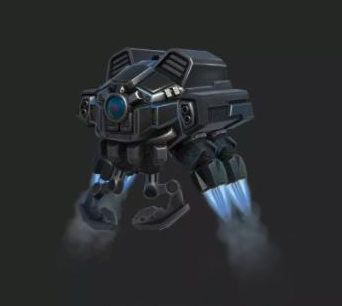
\includegraphics[width=0.5\textwidth]{images/drone.png}
%         \caption{3D Model of our Explorer Drone, from the Unity Asset Store \cite{unity2021}.}
%         \label{fig:cow_fmc}
%     \end{figure}
    
    
% \begin{figure}[!ht]
%     \centering
%     % \subfigure{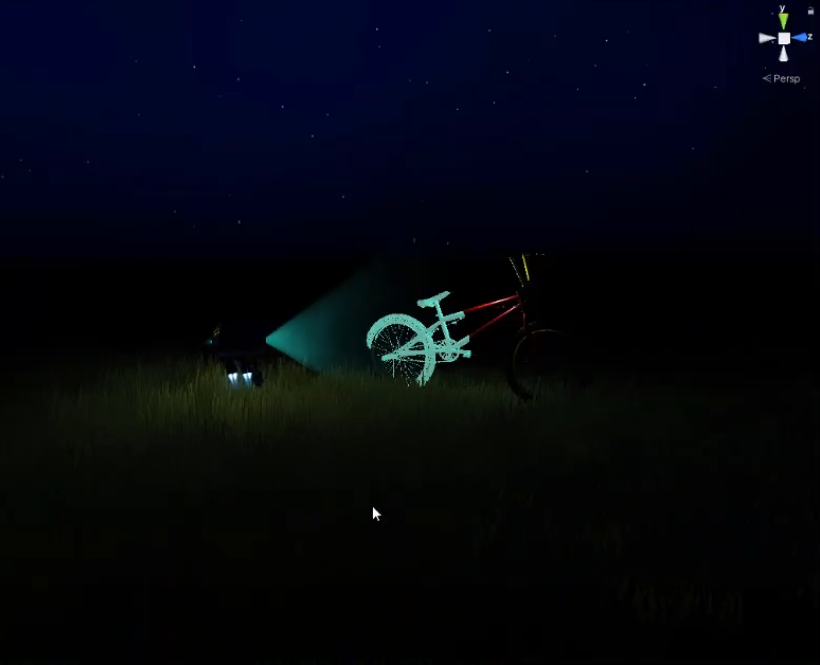
\includegraphics[width=0.315\textwidth]{images/unity-frontpage-drone2.png}} 
%     \subfigure{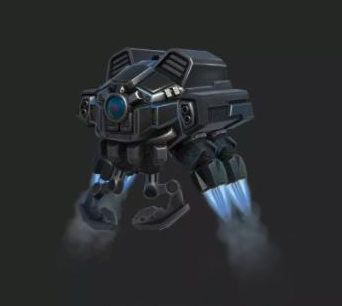
\includegraphics[width=0.287\textwidth]{images/drone.png}} 
%     \subfigure{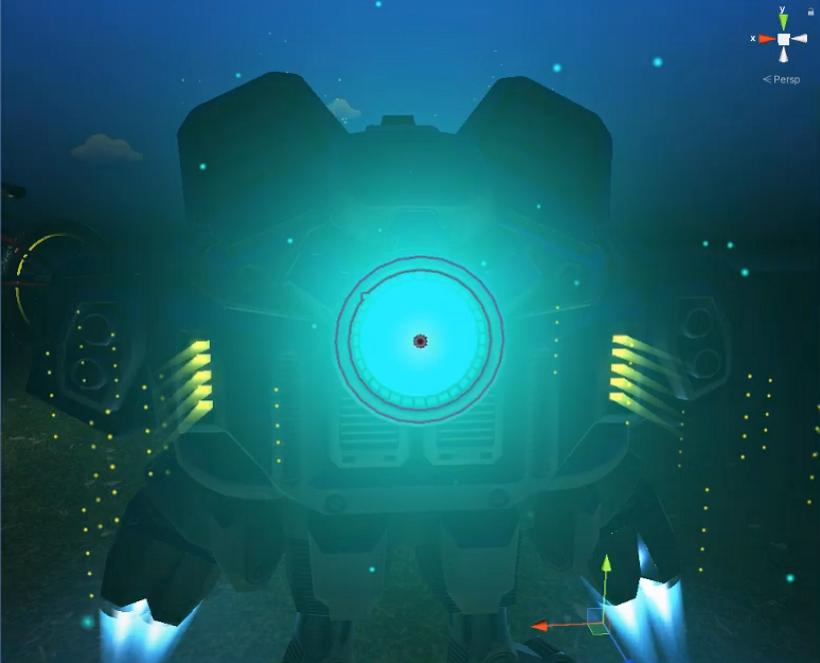
\includegraphics[width=0.317\textwidth]{images/unity-frontpage-drone1.png}} 
%     \subfigure{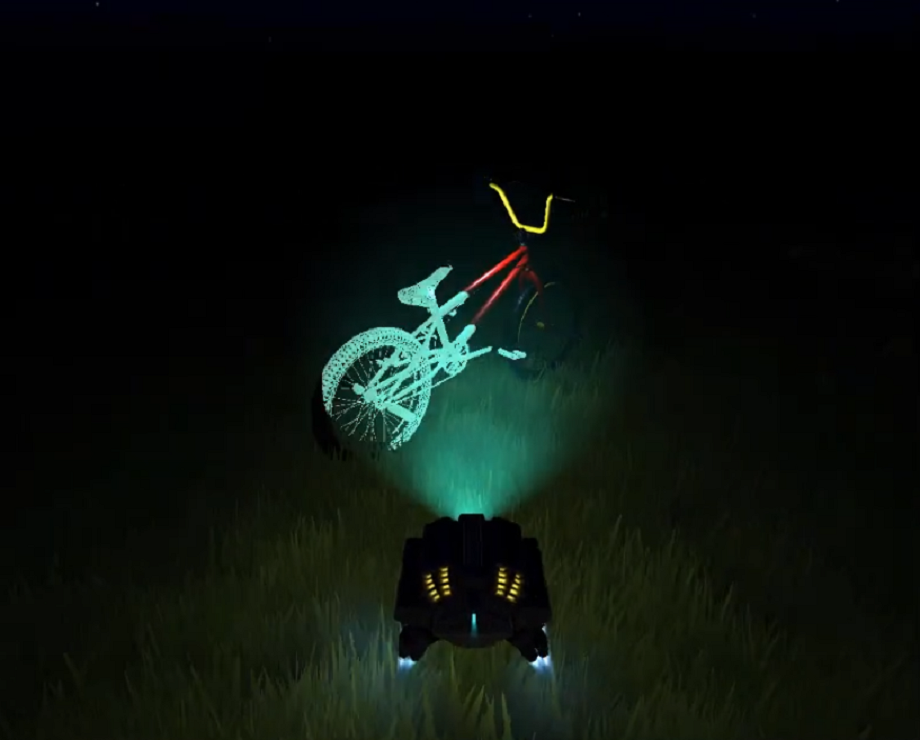
\includegraphics[width=0.32\textwidth]{images/unity-frontpage-drone3.png}}
%         \caption{3D Model of our Explorer Drone, from the Unity Asset Store \cite{unity-asset-store}}
%     \label{fig:frontpage-drone}
% \end{figure}

%  \begin{figure}[!ht]
% \captionsetup[subfigure]{justification=centering}
%     \centering
%       \begin{subfigure}{.49\linewidth}
%         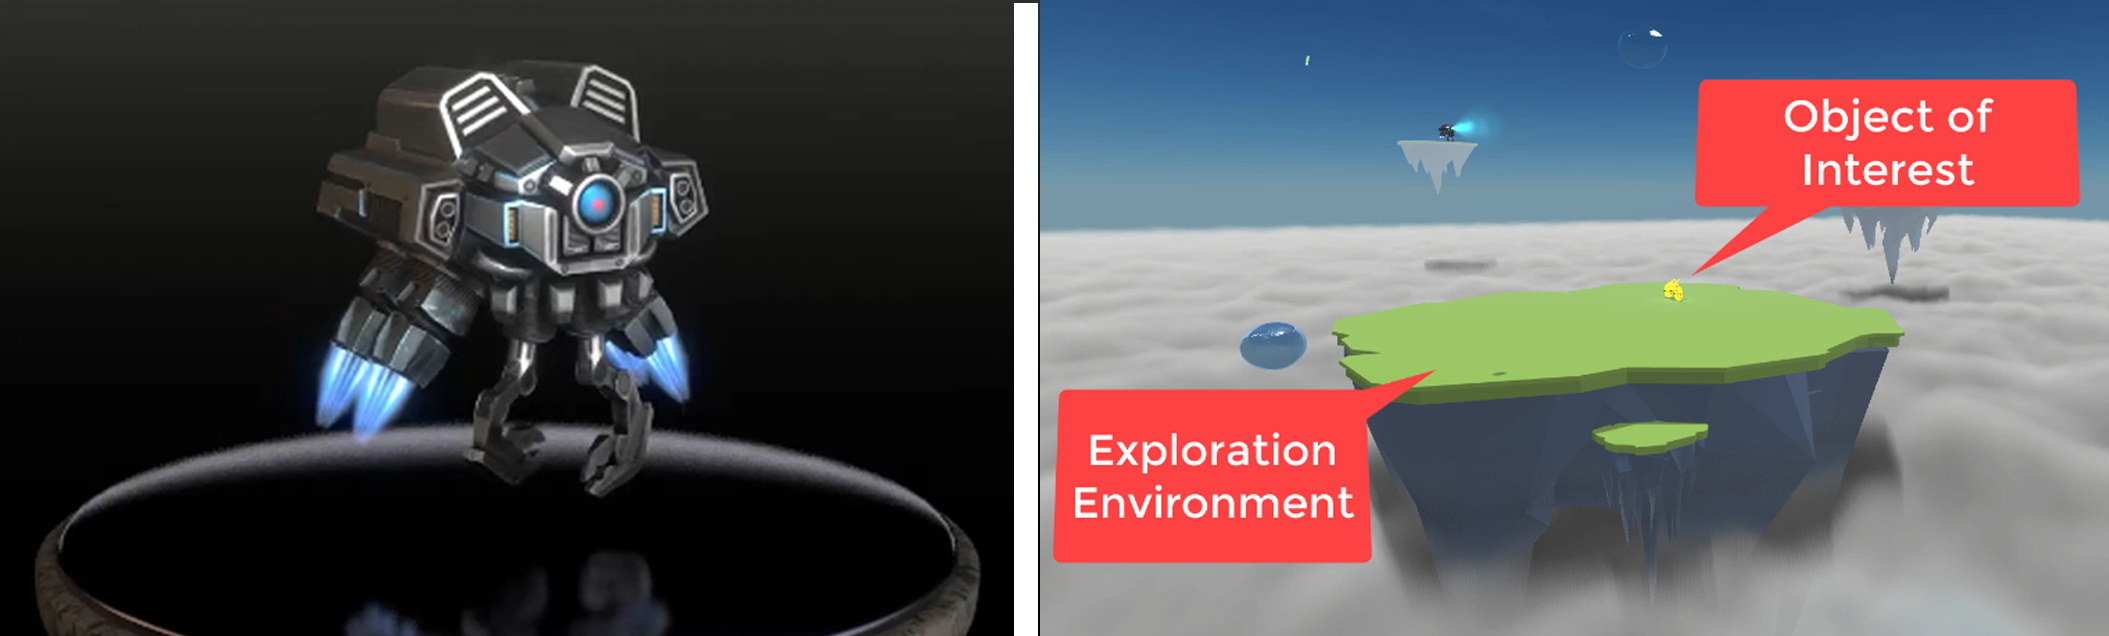
\includegraphics[width=0.5\textwidth]{images/chapter1-figure1.png}
%           \caption{3D Explorer Drone \cite{unity-asset-store} (left) and Training Island (right).}
%           \label{fig:chapter1-figure1.png}
%       \end{subfigure}
%       \begin{subfigure}{.49\linewidth}
%         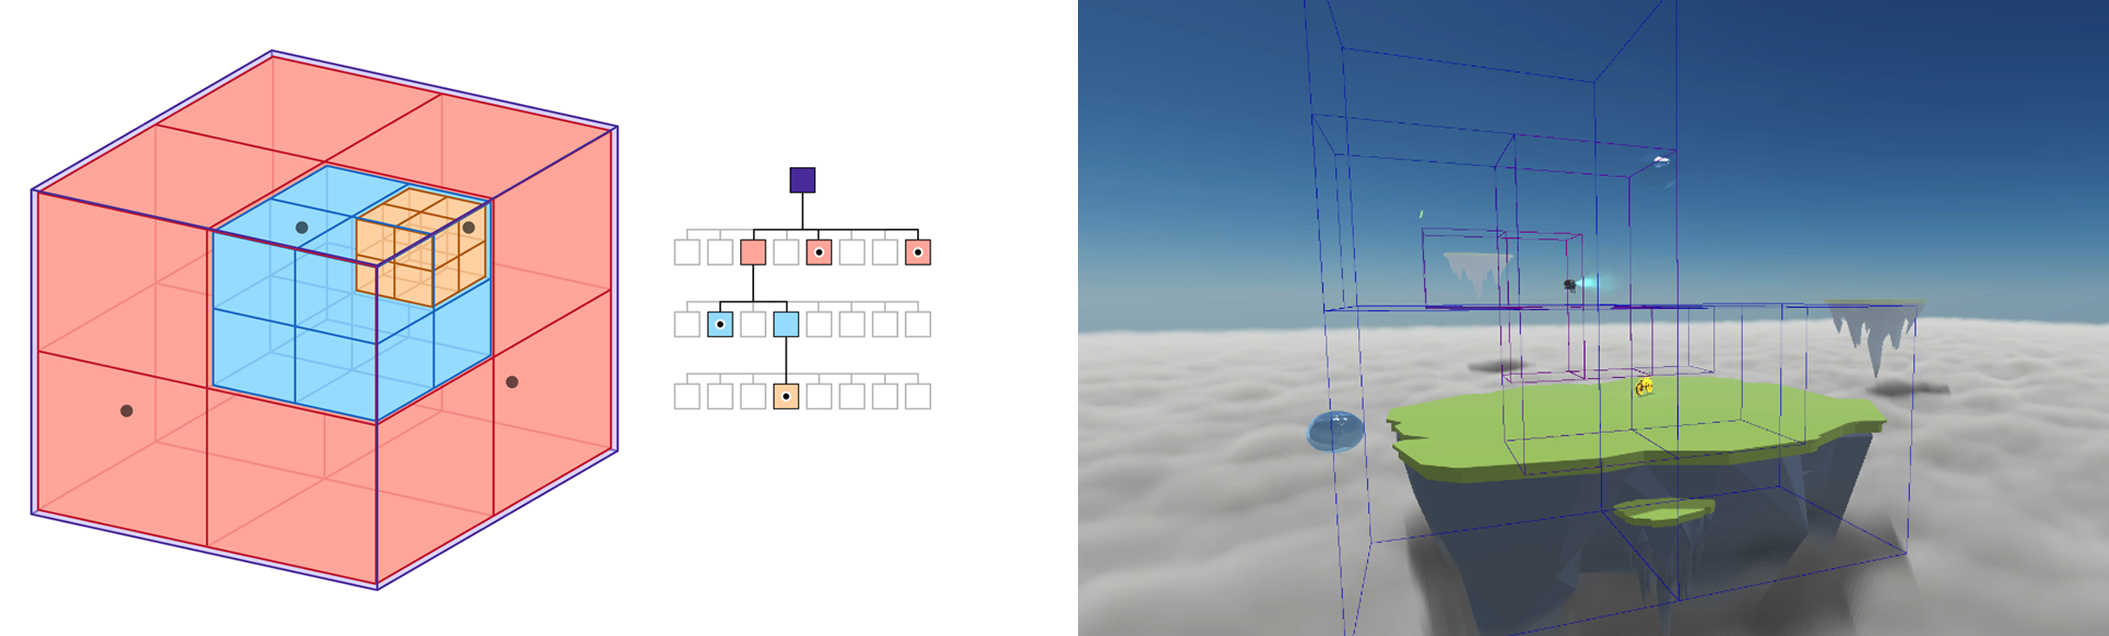
\includegraphics[width=0.49\textwidth]{images/chapter1-figure2.png}
%           \caption{Octree data structure \cite{dulalsaurab_octree} and subdivision \\ of training environment.}
%           \label{fig:chapter1-figure2.png}
%       \end{subfigure}
%       \begin{subfigure}{.49\linewidth}
%         \includegraphics[width=0.49\textwidth]{images/chapter1-figur3.png}
%           \caption{Grid sensor used to enable vision (left). \\ Object of interest and voxel scanner (right).}
%           \label{fig:chapter1-figure3.png}
%       \end{subfigure}
%       \begin{subfigure}{.49\linewidth}
%         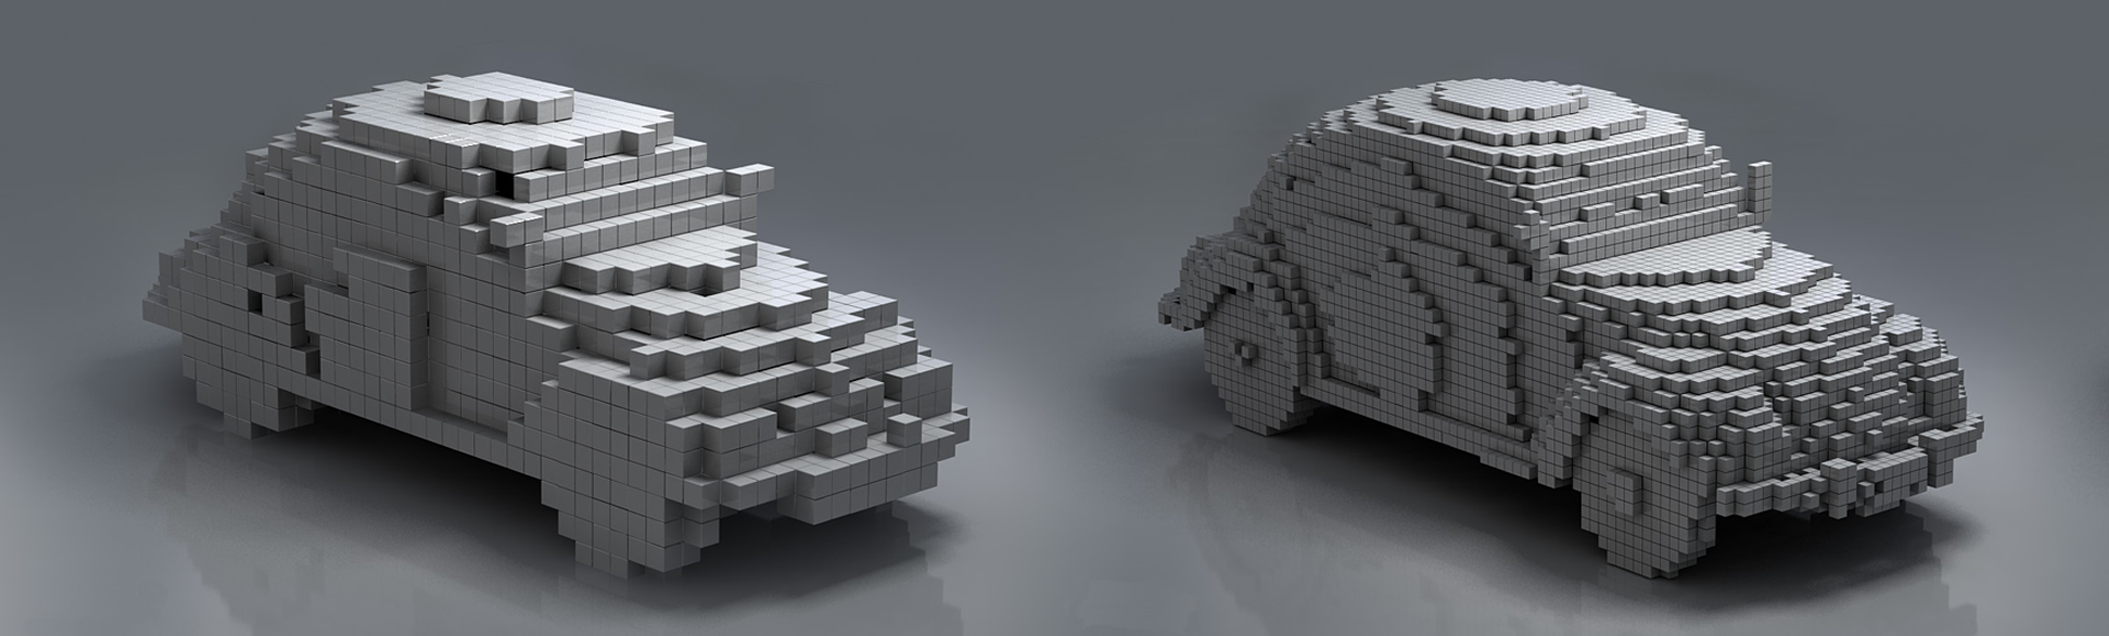
\includegraphics[width=0.49\textwidth]{images/chapter1-figure4.png}
%           \caption{Voxelization of 3D models used to motivate \\ exploration of objects of interest. Taken from \cite{bilderzucht_voxelization}.}
%           \label{fig:chapter1-figure4.png}
%       \end{subfigure}
% \end{figure}



\begin{figure}[!ht]
\begin{center}
    % \subfigure{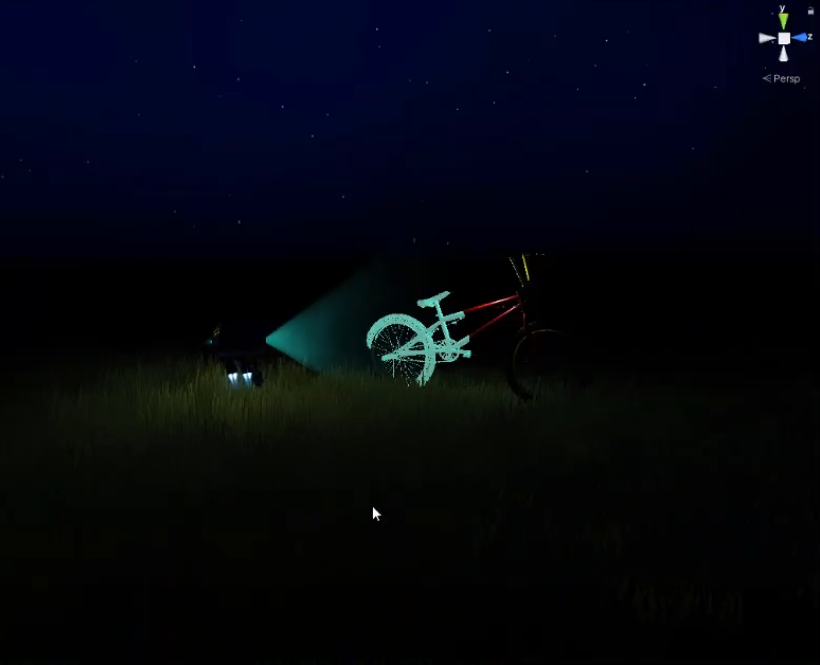
\includegraphics[width=0.315\textwidth]{images/unity-frontpage-drone2.png}} 
    \subfigure[3D Explorer Drone \cite{unity-asset-store}.]{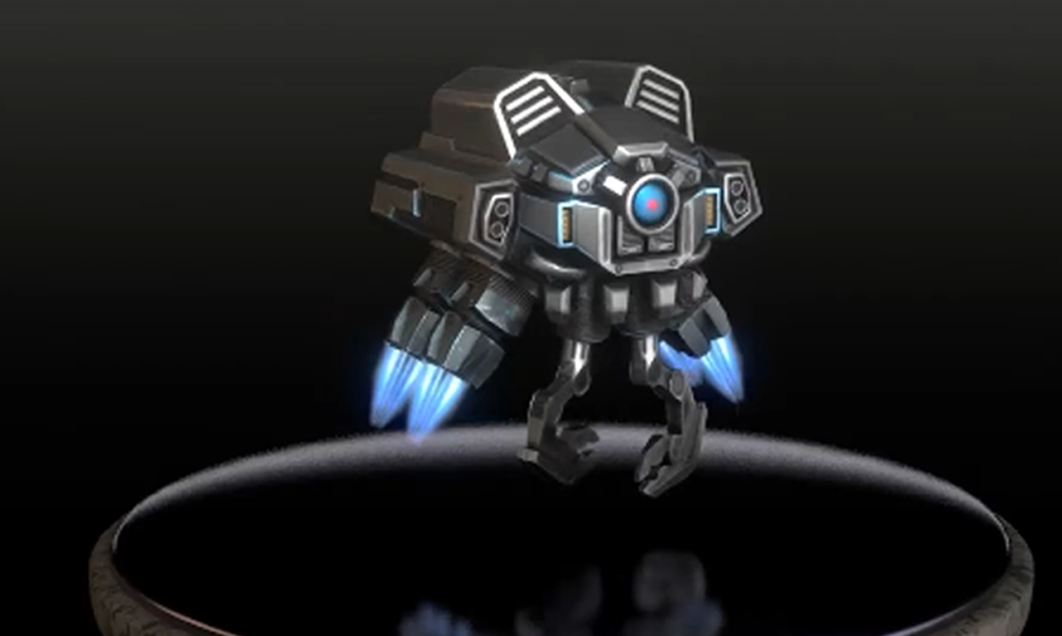
\includegraphics[width=0.245\textwidth]{images/chapter1-small-figure1.png}} 
    \subfigure[Training Island.]{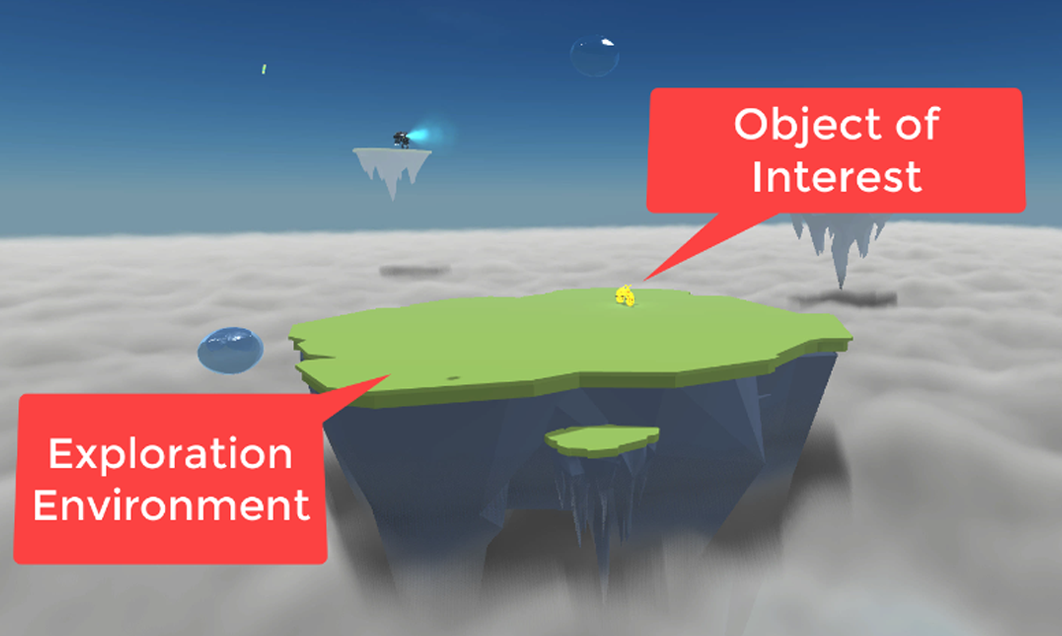
\includegraphics[width=0.245\textwidth]{images/chapter1-small-figure2.png}} 
    \subfigure[Octree data structure \cite{dulalsaurab_octree}.]{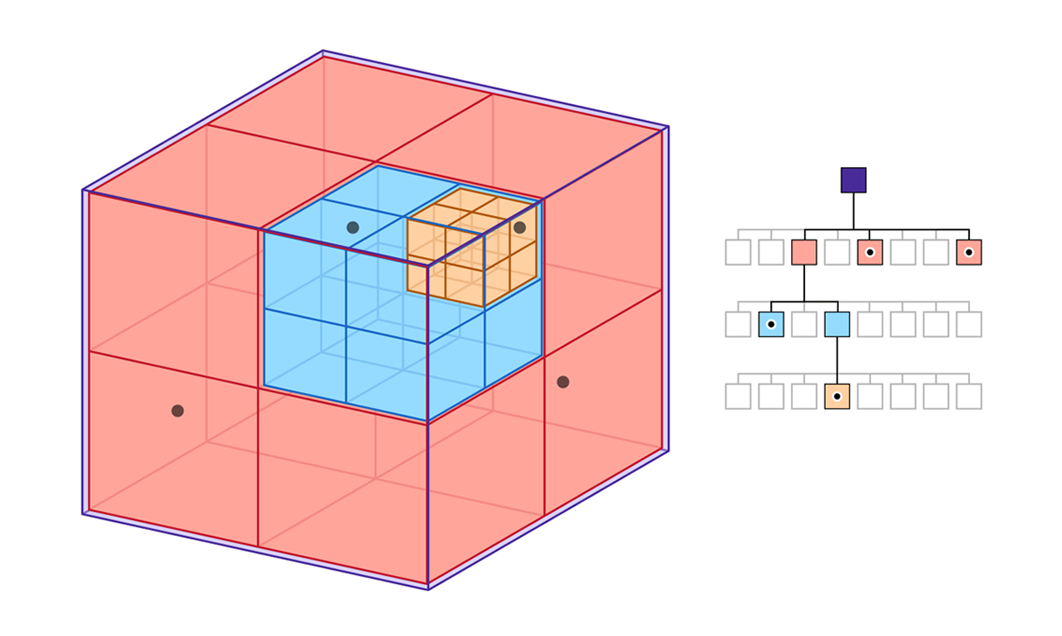
\includegraphics[width=0.245\textwidth]{images/chapter1-small-figure3.png}} 
    \subfigure[Octree island subdivision.]{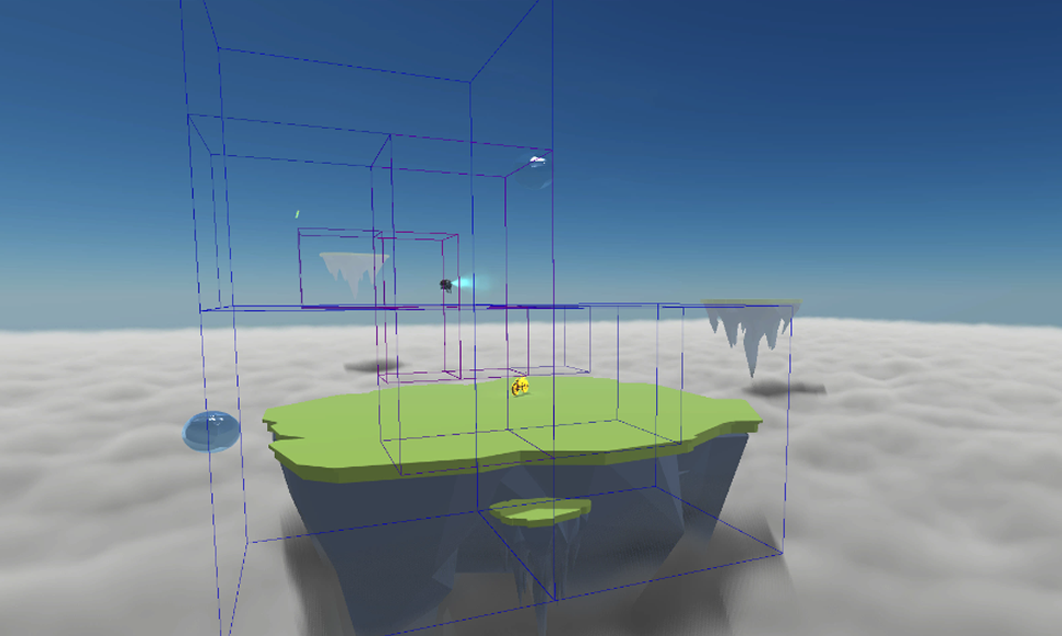
\includegraphics[width=0.245\textwidth]{images/chapter1-small-figure4.png}} 
    \subfigure[Grid sensor for vision.]{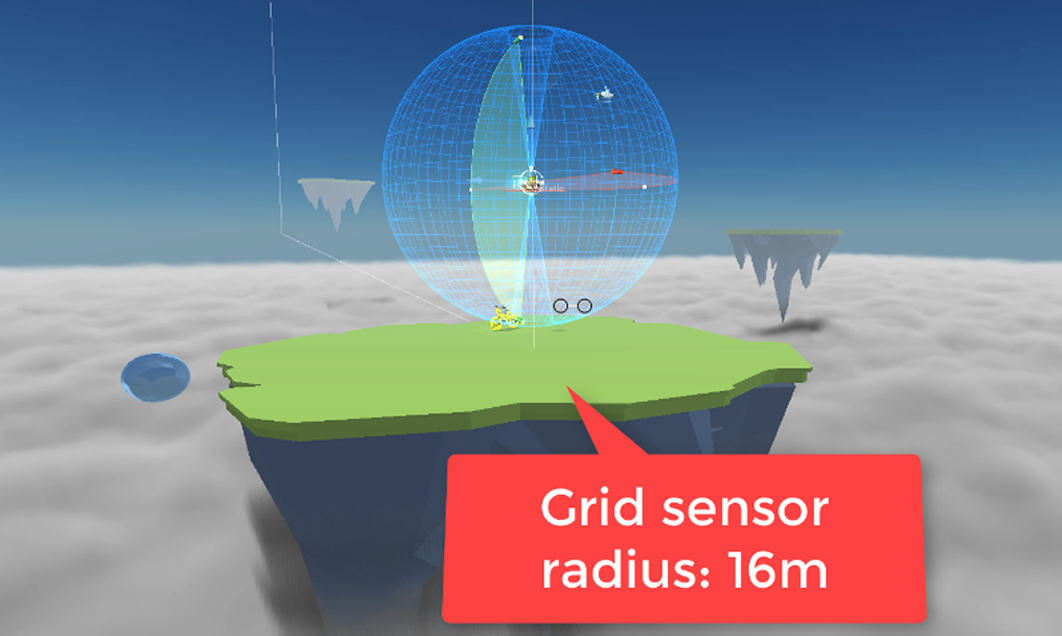
\includegraphics[width=0.245\textwidth]{images/chapter1-small-figure5.png}} 
    \subfigure[Object of interest and voxel scanner.]{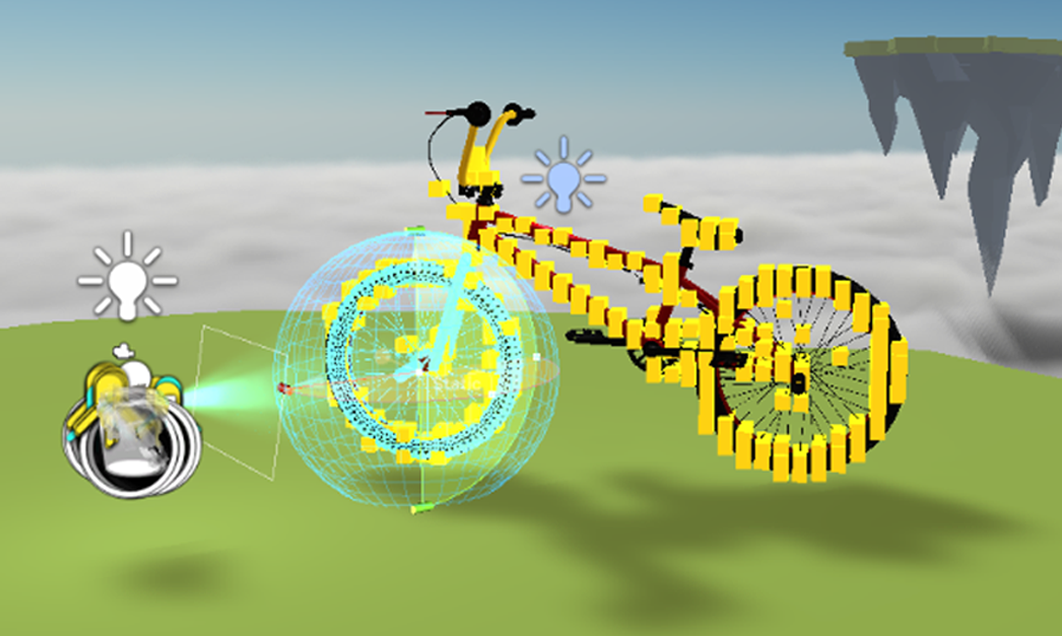
\includegraphics[width=0.245\textwidth]{images/chapter1-small-figure6.png}} 
    % \subfigure[Voxelization used to motivate exploration of objects.]{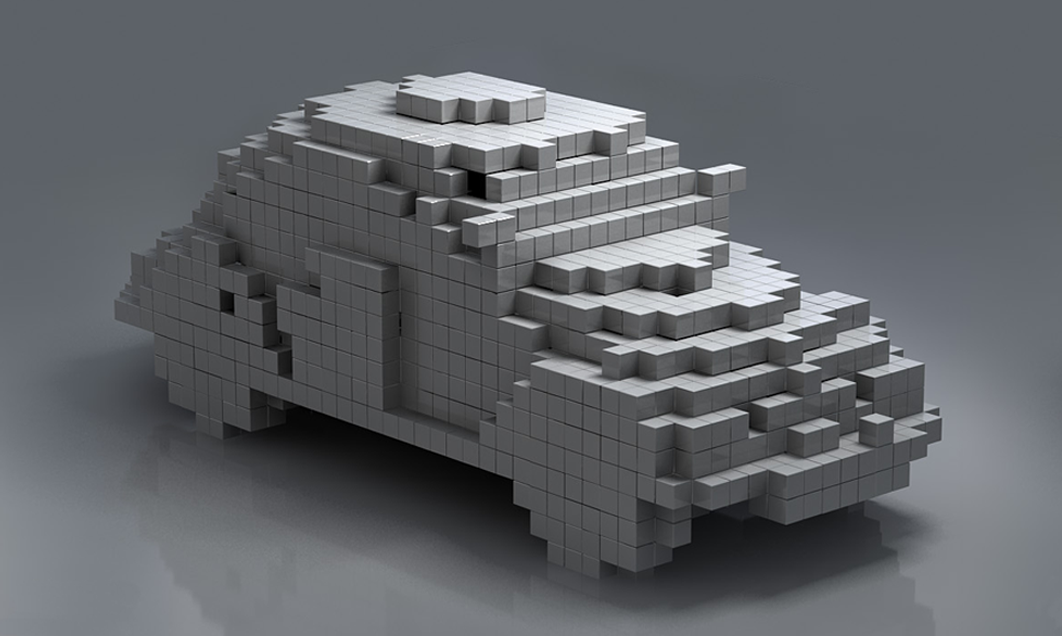
\includegraphics[width=0.25\textwidth]{images/chapter1-small-figure7.png}} 
    % \subfigure[3D Explorer Drone \cite{unity-asset-store} (left) and Training Island (right).]{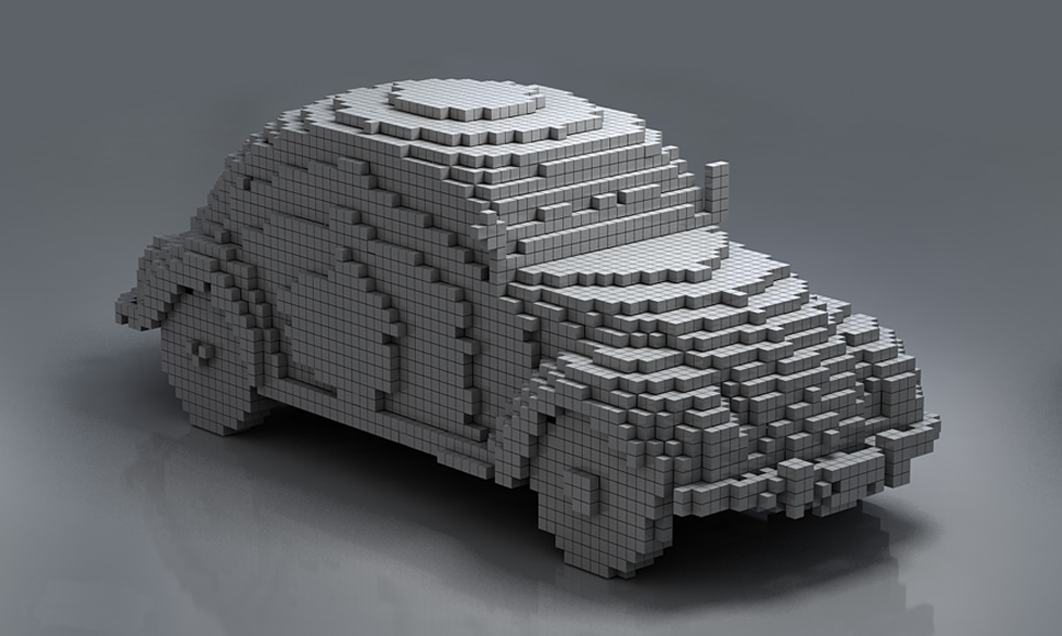
\includegraphics[width=0.25\textwidth]{images/chapter1-small-figure8.png}} 
    \subfigure[Voxelization used to motivate exploration of objects \cite{bilderzucht_voxelization}.]{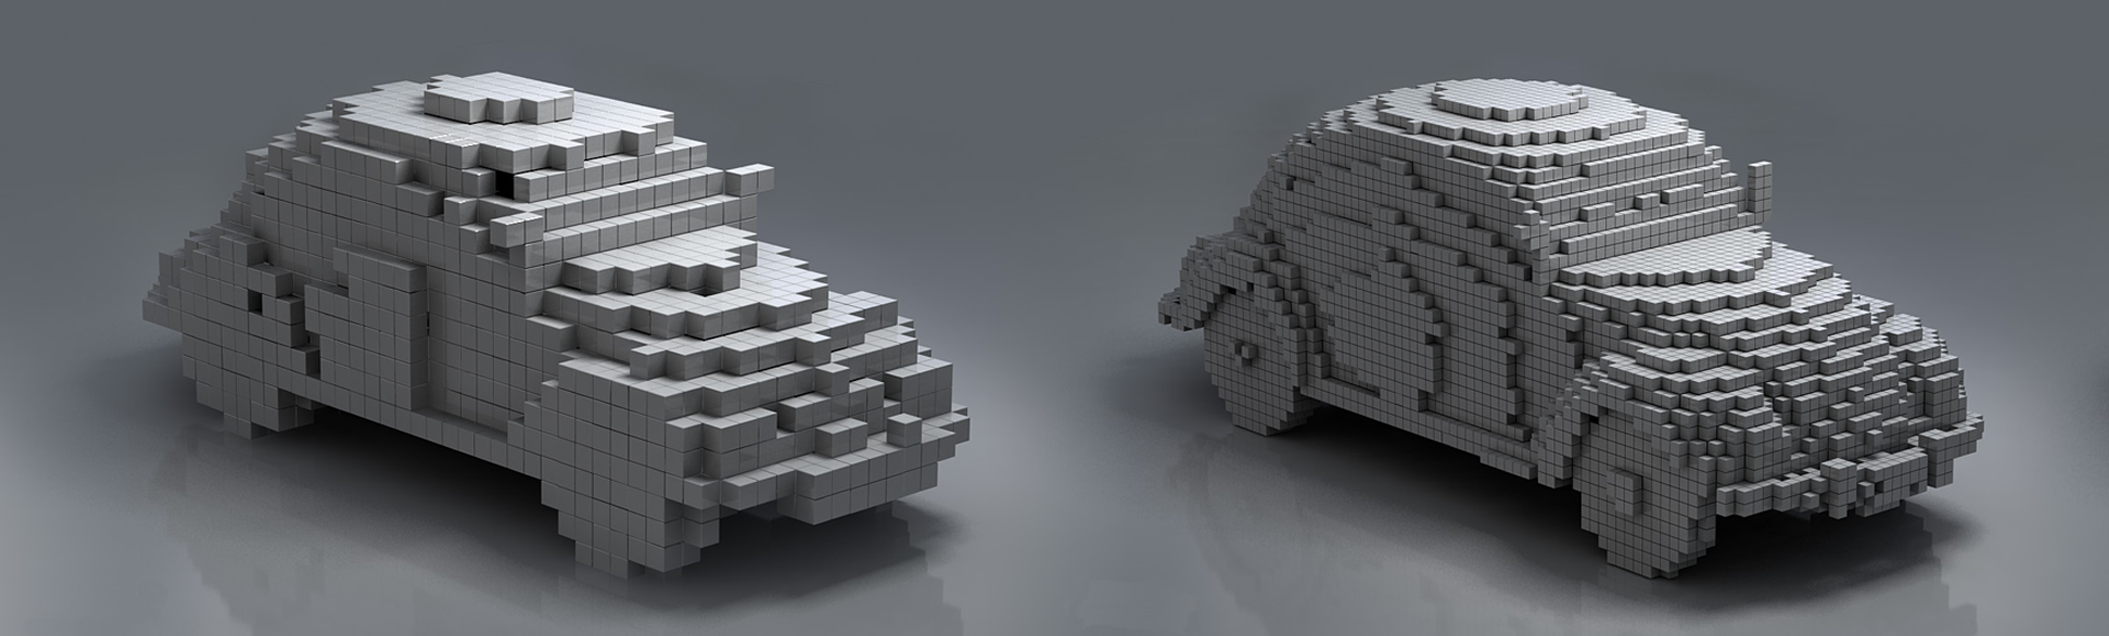
\includegraphics[width=0.49\textwidth]{images/chapter1-figure4.png}} 
    % \begin{minipage}[b]{.5\linewidth}
    % 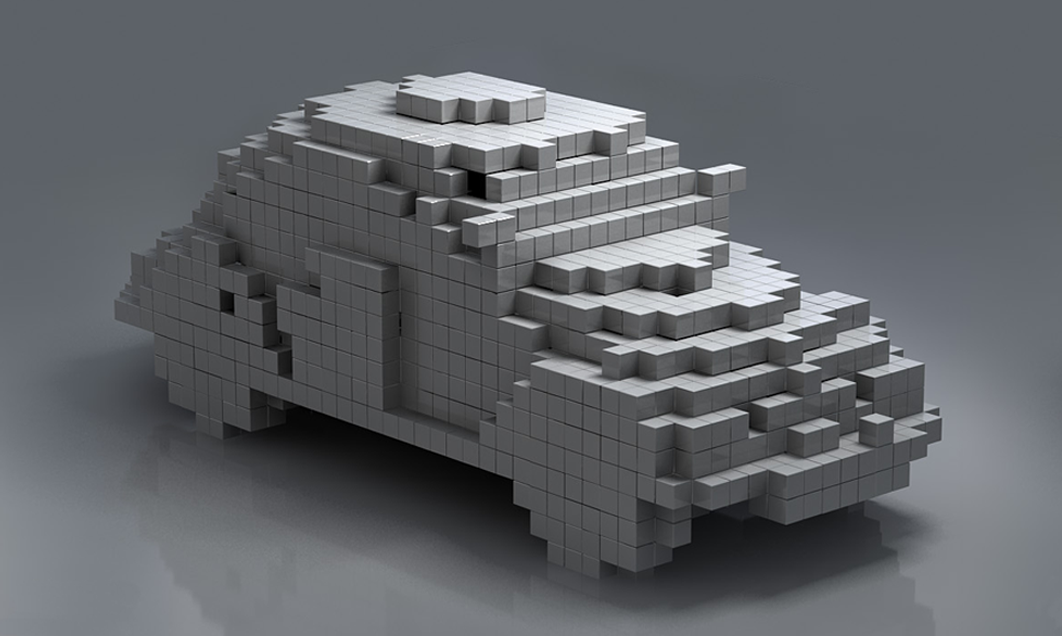
\includegraphics[width=0.49\textwidth]{images/chapter1-small-figure7.png}
    % 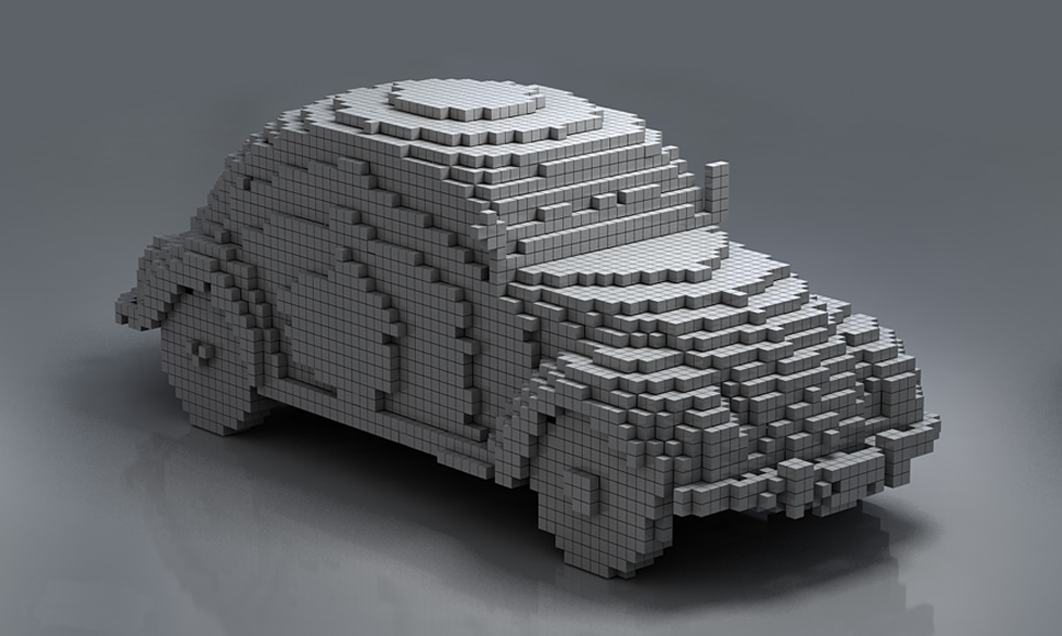
\includegraphics[width=0.49\textwidth]{images/chapter1-small-figure8.png}
    % \subcaption{Voxelization used to motivate exploration of objects \cite{bilderzucht_voxelization}.}
    % \end{minipage}

   
    % \subfigure[ and subdivision \\ of training environment.]{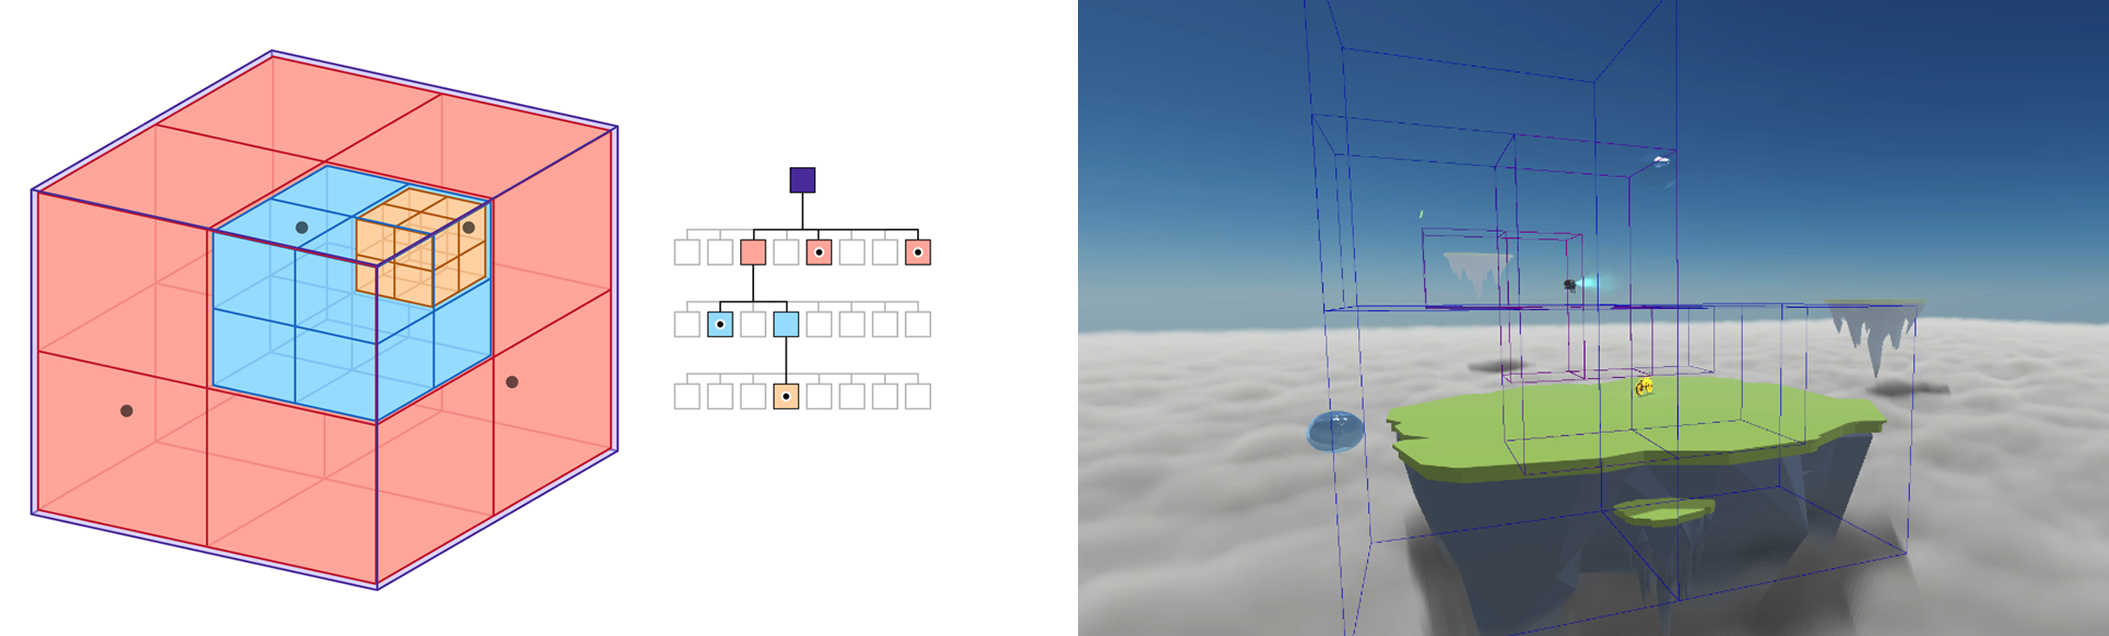
\includegraphics[width=0.49\textwidth]{images/chapter1-figure2.png}} 
    % \subfigure[Grid sensor used to enable vision (left). \\ Object of interest and voxel scanner (right).]{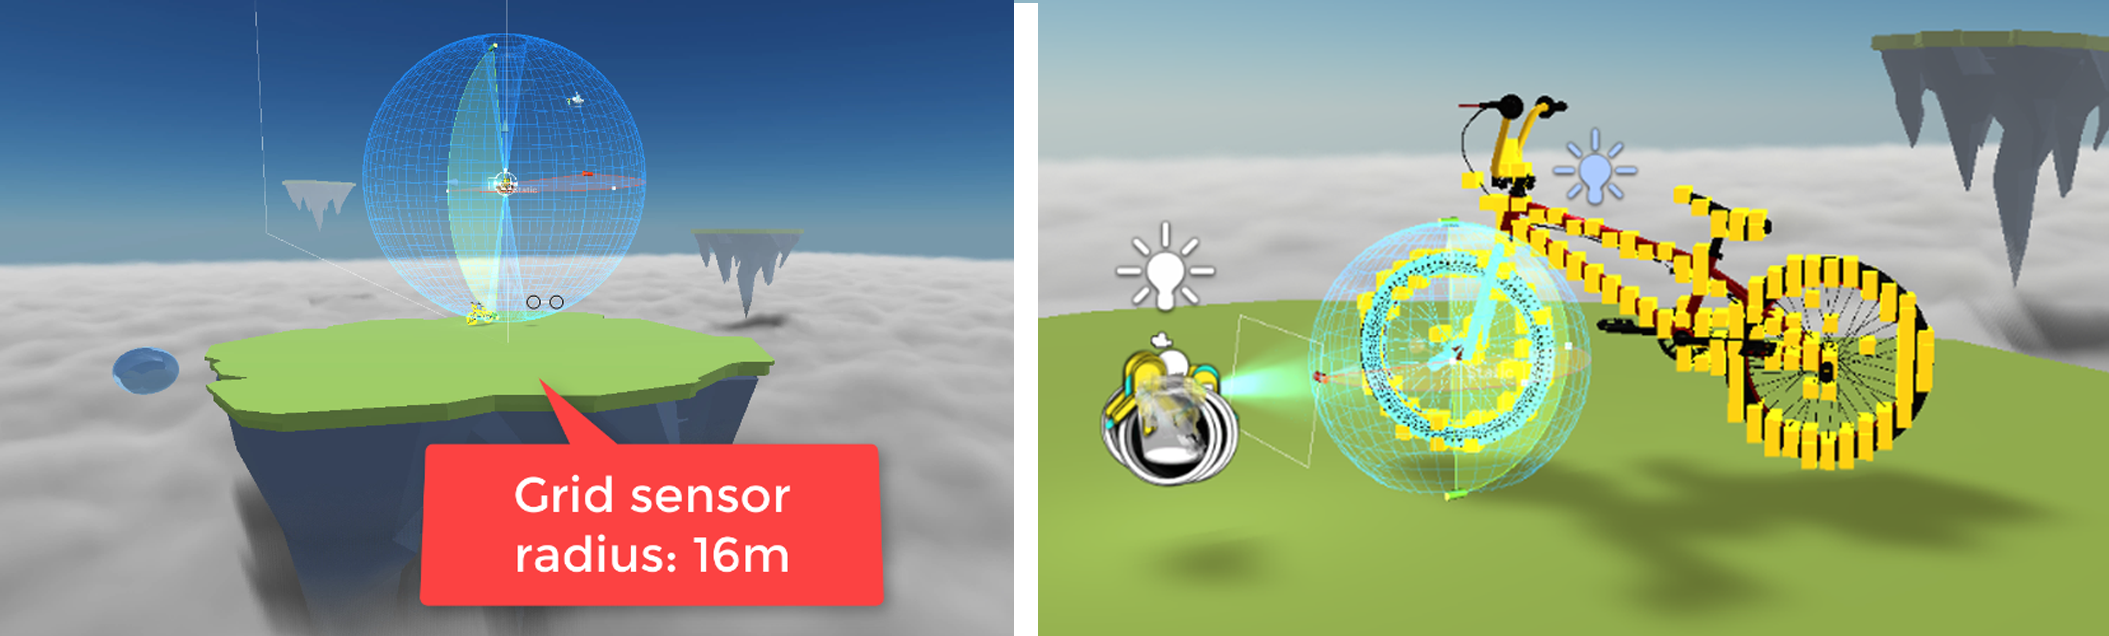
\includegraphics[width=0.49\textwidth]{images/chapter1-figure3.png}} 
   
    % \caption{3D Model of our Explorer Drone, from the Unity Asset Store }
    \label{fig:frontpage-drone}
\end{center}
\end{figure}

\section{Motivation}\label{chap:1:motivation}
% Use Case: Improving the Cow Milking Automation
% - first time scene understanding was done
% - scene understanding today and what value it has for enterprise applications
% - current state of scene understanding
% - limitations / challenges / problems with it

At the NeurIPS 2017, \textcite{abbeel_youtube_2017} presented a video of robots cleaning a living room, bringing a bottle of beer, and performing tasks usually seen in science fiction movies.
Later it was showed that the robot was being controlled by a human with a remote controller: his presentation hinted towards the fact that the robots that we use today are physically capable of performing such actions, so building state of the art robotics is not a hardware problem anymore but a software one.
As of 2021, tasks like teaching a robot how to pick a bottle of beer can still be a very challenging task. Nevertheless, current algorithms have come a long way since Pieter's talk and much has been done to improve robots' understanding of their environment and to study what set of tools are required to achieve not just perception in robots but intelligent agents \cite{kok2020trust, trivedi2008soft}.
Works like DeepMind's recent publication \cite{silver2021reward} hint towards a promising future where reward maximization methods are a promising path towards general artificial intelligence. Where current AI models outperform humans at specific tasks and alleviate repetitive workloads, general AI would potentially outperform humans at nearly every cognitive task. 
It is therefore imperative to continue research in disciplines such as reinforcement learning as it is one of the most promising field to achieve intelligent robotic behavior \cite{song2021autonomous, abbeel_youtube_2017, kok2020trust, silver2021reward}.

% is of vital importance to to eventually

% most common ML applications people use supervised learning (input, and know what the output is, so we can use an optimization algorithm to compute gradients to train the NN to produce the outputs)
% - (rewrite) In this sense, applications that use these kind of technologies are scarce given the lack of [...] and [...].

% It is believed that the first time a cow was milked was around 8,000-10,000 years ago, somewhere in Europe\cite{valente_2017}. Interestingly, milk also is given the credit for the developments that have happened in the modern food industry. Not only because of how widespread it is in today's culture, but also because of bringing cheese and butter with it. Over the past 8,000 years, more than a handful of technological advancements have happened, specially in the farming industry. The Agricultural Revolution proved to be a turning point for the food supply, allowing the way for the Industrial Revolution \cite{lumenlearning_2021}. Consequently, milking robots have been around in agriculture for over 20 years. However, the concepts of the widespread milking systems available on the market have hardly had any adaptations leveraging the latest technological advancements. The current largest supplier, Lely, still uses electro-pneumatic spindle motors even in the latest version of the milking robot (Astronaut A5). The benefit of these motors is their low cost and their physical compliance, making them resistant to cow kicks. They require, however, a lot of maintenance. For example, the seal of these motors must be replaced regularly so that the system remains operational. As of today, the herd size in Swiss farms is often big enough so that more than one milking robot would be needed, but the space requirements do not allow for this without having to remodel the barn's infrastructure.

% TODO adapt this part to be in line with scene understanding

Accordingly, a current project at ZHAW linked to this thesis work aims to construct a milking robot that leverages machine learning methods to outperform traditional milking robot technologies, in cooperation with the industrial partner Sutter Landtechnik GmbH (SLG).
Most of today's milking robots use a 2D laser scanner to estimate the position of the cow, the udder and the cow's teats, and several measurements are necessary. This is time consuming and if the cow moves during the measurement, the position estimation must be reinitialized. ZHAW therefore proposes innovative changes to the milking robot's architecture, using electric drives and a more compact kinematic structure. Moreover, given that inexpensive 3D cameras have been introduced to the market over the past few years, it is now possible to leverage high resolution 3D point clouds to dynamically estimate the position of the cow teats while also reducing the costs of manufacture. 

This thesis aims to contribute to this project but also to the fields of practical reinforcement learning, computer vision research and practical machine learning. To this end, we abstract the scenario of a milking robot as an unknown environment with objects of interest, a reinforcement learning agent's task is to explore such an environment and the objects in it.
% the milking robot problem represents an unknown environment where not only the position of objects is of interest, but the general level of awareness of the overall environment itself.
In other words, the aim of this masters thesis is to select and implement a computer vision enabled pipeline that leverages active vision to reduce the uncertainty over time in a new environment, one of which can be a milking robot's environment. In this sense, uncertainty is defined as the amount of unscanned voxels in the scene, the unexplored locations and the measured temporal semantic entropy given by an object detector.
%  and the derived class complexity through the Shannon entropy. 

The proposed solution is inspired by the human brain's physiology and approximates the discovery process a human would follow in an unknown environment. It also leverages the concept of temporal semantic entropy proposed by \textcite{chaplot2020semantic} to define this dimension of uncertainty. Concretely, the task at hand is exploration for coverage maximization, for which we propose a novel approach that leverages extrinsic rewards from voxel scans constructed from ubiquitous RGB-D information. From the perspective of architecture design, it proposes a pipeline that can be further extended to a multitude of use cases and even other semantic models, in an attempt to contribute to the research on semantic-curiosity-motivated exploration.

Finally, while there are increasingly more 3D datasets out there for benchmarks on computer vision tasks, reinforcement learning algorithms have seen themselves limited to black box environments and popular games such as Atari 2600, Quake III, Doom, Minecraft and Gazebo simulations. However, as deep reinforcement learning algorithms become more sophisticated, new environments and benchmarks must emerge since existing environments and benchmarks based on them become less informative \cite{juliani2018unity}. This work contributes to existing agent testing environments with three 3D Unity-based scenarios, which are easy to extend to further use cases. They also differentiate themselves from traditional benchmarks by being developed with improved realism, which aims to close the gap between synthetic and realistic data. These environments are used to further evaluate the exploration task at hand and the feasibility of knowledge transfer across environments. All of this leaves the door open for future research in simulated applied vision systems and for in-robot implementations of the exploration policies studied.

% Based on this background, the aim of this Masters thesis is to select and implement a machine learning and computer vision enabled pipeline that estimates the 3D pose and direction of cow teats. The methods proposed in this work build the basic structure for an approach to estimate the position of the cow teats.



% Unity: A General Platform for Intelligent Agents
% As deep reinforcement learning algorithms become more sophisticated, existing environments and the benchmarks based on them become less informative. For example, most
% environments in the ALE have been solved to above human-level performance, making the
% continued use of the benchmark less valuable (Machado et al., 2017; Puigdomènech Badia
% et al., 2020). A complementary point created by this state of algorithmic progress is that
% there exists a virtuous circle in which the development of novel environments drives the
% development of novel algorithms. We can expect the research community to continue to
% provide high-quality algorithms. However, it is unclear from where researchers should expect
% high-quality environments, since the creation of such environments is often time-intensive
% and requires specialized domain knowledge. This continual need for novel environments
% necessitates an easy-to-use, flexible and universal platform for unrestricted environment
% creation.
% Simulated environments are constrained by the limitations of the simulators themselves.
% Simulators are not equal in their ability to provide meaningful challenges to learning systems.
% Furthermore, it is sometimes not obvious which properties of an environment make it a
% worthwhile benchmark for research. The complexity of the physical world is a primary
% candidate for challenging the current as well as to-be-developed algorithms. It is in the
% physical world where mammalian and, more specifically, human intelligence developed, and
% it is this kind of intelligence which researchers are often interested in replicating (Lake et al.,
% 2017).

% Although this requires much more complex data processing on a powerful control system, it does away with a time-consuming, separate 
% time-consuming, separate measurement process can be dispensed with. Dynamic measurement with modern sensors also offers the potential to be much more robust and reliable than the measurement methods used today.
    
    % \begin{itemize}
    %     \item describe the general need for automated cow milking
    %     \item describe how the problem is currently being solved briefly
    
    %     \item describe the challenges in cow teat recognition: morphology/shapes and movement
    %     \item describe how these methods fail || describe challenges/limitations of current methods (sensors, etc, no memory)
    
    %     \item can solve this problem with computer vision briefly
    
    %     \item describe cow project main driver (The InIT's purpose) (do we mention how expensive current solutions are?)

    % \end{itemize}
% \section{The Need for Organic Milk}\label{chap:1:organic-milk}

% In recent years, the financial pressure on agriculture in Switzerland has increased massively. Since 1980, the number of farms has been shrinking by about 1000 farms per year. The Swiss consumer wants more and more organically grown products and at the same time consumer prices are getting cheaper and cheaper. The extensive Swiss animal welfare regulations, which are the strictest in Europe, make animal husbandry even more expensive. All this leads to the fact that the average income of a farmer family decreases annually. The farmers' association is therefore calling for greater support from the state. The SLG sees the key to running a profitable Swiss farm not in higher government subsidies, but in a more efficient machine park, which is specifically optimized for the Swiss market, according to Swiss legislation and for organic and ecological farming. All robotic milking equipment available today is not designed for organic farming but optimized to maximize milk yield. However, in the saturated Swiss milk market, what is needed is not more milk, but rather milk produced in a fair, organic and cost-efficient way.

% Across Europe, organically produced milk is still a niche product. However, the SLG is convinced that this will change in the coming years, as consumers in Europe are also paying more and more attention to what they eat and how their food was produced. The focus of a new development should therefore not be on maximizing the amount of milk per animal, but on minimizing investment and operating costs, and above all, these new systems should enable organic farming without compromise. This starts with giving cows access to pastures.

% Today's robotic systems are designed for 24/7 operation. Especially for smaller farms, this mode of operation is necessary to keep operating costs low. In contrast, an important feature of the new robotic system is to be able to milk all cows on a farm within one to two hours, thus combining all the advantages of a conventional milking parlor with the benefits of a milking robot. For this purpose, the new robot is dimensioned in such a way that several robot arms can be installed in the intermediate aisles of existing barns without the need for major cost-intensive building adaptations. By installing the robot in the intermediate aisles of the barn, it will also be possible to minimize the use of concentrated feed, as the cows will automatically pass the robot when moving from the cubicles to the feeding axles.


\section{Purpose and Research Questions}\label{chap:1:research-question}
% In this work, a machine learning and computer vision based solution will be used to estimate the pose of cow teats for a milking robot. Regarding this task, this work tackles the following research question:
% How can the cow teats 3D pose be estimated under 10 seconds?
In this work, the problem of uncertainty in an environment presented by the milking robot is looked from a more general perspective. We therefore look at exploration policies that can also contribute to a plethora of other use cases. More concretely, we propose a reinforcement learning based solution to explore a 3D scene and the objects in it. To this end, we use extrinsic motivation while also leveraging the uncertainty in the environment to adapt such behavior.
% maximize coverage in a 3D scene, using extrinsic motivation to pursue new states.
% new environments. 
% Moreover, it takes into account uncertainty in the environment, defined by the temporal inconsistencies in an object detector as a supporting exploration metric. 
Finally, a set of research scenarios are proposed to show the versatility of our exploration policies and contribute to existing benchmark environments. 
% and account for realism using Unity 3D
Regarding this task, this work tackles the following research questions:
\begin{itemize}
      \item How can an embodied agent increase the overall certainty about an object's characteristics, i.e., how can trajectories around objects of interest be covered to reduce the uncertainty about such objects? 
      \item How can these objects be found in large and unknown environments by the same agent?
\end{itemize}

% \begin{itemize}
%     %  Howcan an active vision exploration policy based on a ubiquitous source of information such as voxels, in currently accessible RGBD cameras, contribute to reducing the uncertainty about a scene?
%     % \item How can voxel structures be exploited for intrinsic motivation in active vision exploration policies?
%     % \item How can uncertainty, defined through semantic entropy, be used to thoroughly scan objects through active vision policies?
%     % \item How can active vision exploration policies be leveraged for a practical scenarios, beyond the original milking robot use case? 
%     % 3D data (meshes or point clouds), in voxel form, be exploited for extrinsic motivation of objects?
%     \item How can an embodied agent increase the overall certainty about an object's characteristics, i.e., how can trajectories around objects of interest be covered to reduce the uncertainty about such objects? 
%     \item How can these objects be found in large and unknown environments by the same agent?
%     % \item How can uncertainty be defined through semantic entropy and be used as a motivation in exploration policies?
    
% \end{itemize}

\section{Approach and Methodology}\label{chap:1:approach-methodology}
This work focuses on leveraging reinforcement learning techniques to manipulate an agent (camera) motivated by abstractions of the perceived environment. These abstractions are meant to simplify the complexity present in the environment and take the form of translations of camera input into voxels. Voxels, accordingly, represent the direct goal for a scanning agent to obtain view from an object from multiple angles. The problem that is further studied within this master's thesis is two-fold: 1) uniform exploration of large open spaces and 2) thorough scanning of objects from multiple angles, as a mean to reduce the uncertainty in a 3D scene over time. We define, therefore, uncertainty through the semantic entropy observed at a given point in time, which is inspired by \textcite{chaplot2020semantic}.

The strategy taken for this project work is the following:

A state of the art analysis was done to propose a set of exploration policies using reinforcement learning that answer the research questions. 
First, this analysis includes the evaluation of related efforts in scene understanding, active vision, and RL-based exploration.
% variety of advancements in computer vision and machine learning fields such as 3D data representation, object detection, scene understanding, and reinforcement learning techniques for the manipulation of a vision-driven agent for exploration.
% pose estimation for the 3D pose estimation of cow teats.
% This also includes the implementations of the proposed algorithms and the respective optimization of their parameters to solve the task optimally. 
Second, it includes implementations of exploration policies and the respective optimization of the learning environment and the learning agent and its algorithm to solve the task optimally. 
It is also important to note that this process has an iterative nature, where the validation of the models' results triggers changes for optimizations in the learning environment and the agent, 
% , and the diverse algorithms' parameters
in order to achieve the best possible results. The used data is of synthetic origin, and was modeled, assembled and simulated in the Unity game engine. Finally, the results were critically evaluated and compared to a set of baselines. The generalization capabilities, reliability and limits of the results are then discussed and further improvements on this field considered. 
%  further work: using semantic queues, implementing full pipeline using RGB to measure how computation heavy the voxel calculation could be and optimization strategies, a.k.a. out of scope limitations that will only be discovered when the actual voxel manipulation is done (work by RoutedFusion and seems promising to work on scans). 

\section{Contributions}\label{chap:1:contributions}
Our contributions can be summarized into the following points:
\begin{itemize}
    \item We build upon knowledge acquired through a previous publication, namely \textit{\citetitle{DBLP:journals/corr/abs-2105-09843}} \cite{DBLP:journals/corr/abs-2105-09843} and the Bachelor's thesis \textit{\citetitle{dano2020}} \cite{dano2020}, to propose a novel voxel-based exploration method, which builds upon model-free
    % to the best of our knowledge
    reinforcement learning
    % to enable visual-agnostic exploration
    and accounts for the abstract concept of "uncertainty" in an environment, defined through the amount of different object classes present in such an environment. This definition is known as "semantic entropy, or as "the inconsistencies in the temporal class density", as inspired by the concepts presented by \textcite{chaplot2020semantic}.
    
    \item We demonstrate that our method outperforms our Unity implementations of classical and geometric exploration for scanning strategies, and further improves upon exploration methods motivated by coverage maximization \cite{chen2019learning} using octrees and adapts its exploration pace through semantic entropy.
    % , which is inspired by \textcite{chaplot2020semantic}'s semantic curiosity. 
    
    \item We show that Proximal Policy Optimization (PPO), with minimal hyperparameter tuning and any domain-specific algorithmic changes or architectures, achieves final performances and converges faster than the Soft Actor-Critic algorithm \cite{schulman2017proximal}.
    %   comparable to the
    % where  synthetic data and real data for the exploration of 3D environments
    \item By using voxels and grid sensors for extensive exploration, our method abstracts the complexity in the 3D world through voxels and therefore is capable of visual-agnostic exploration and transfer learning tasks. 
    % data distribution plays a key role in the performance of transfer learning techniques trained on synthetic data and tested on real robots, enabling the agent to adapt to new environments without changes in its behavior.
    
    \item We evaluate our approach through relevant statistics for exploration and for thorough scanning of objects, where a set of baselines were defined and two DARPA-inspired evaluation environments \cite{darpa_subterranean_challenge} were implemented.
    % inspired by .
    
    \item We further demonstrate that our method excels in new 3D scenarios that represent real life situations where exploration time is critical to save not just time and costs but, more importantly, lives and further losses. 
    
    \item We present the capabilities of Unity-based environments for the development of new benchmarks and its compatibility with the OpenAI gym platform \cite{openaigym} and trainers from Stable Baselines 3 \cite{github-dlr-rm-baselines3}. 

    \item Finally, we demonstrate that an agent equipped with panoramic vision outperforms agents with ordinary monocular vision in the given exploration task, inspired by \textcite{rill2021collision, wojek2012monocular}.
    % Finally, with an ever increasing amount of algorithms, traditional benchmarks become uninformative and allow room for the creation of newer ones capable of testing more sophisticated challenges, representative of the real world. Motivated by recent works in the Unity 3D engine, we contribute three hyper-realistic 3D environments that can be extended for the creation of new benchmarks, testing of new exploration methods and for a variety of other tasks such as synthetic data generation, autonomous driving, exploration, navigation, point-to-goal tasks, etc. The code base for our method can be found at \url{https://github.com/Ademord/ma-unity}.

\end{itemize}

\section{Scope and Limitation}\label{chap:1:scope}
Due to the time constraints, some limitations were laid out to ensure the work was finished within schedule.
\begin{itemize}
    \item The approach used focuses on the manipulation of synthetic data, namely, 3D voxels in the Unity Engine, while the manipulation of point clouds to generate these voxels is left out. This allows the masters thesis to focus on the research on exploration policies for scanning of objects than on computer vision methods for point cloud manipulation.
    \item This work focuses on the results observed in computer vision and machine learning approaches limited to models compatible with the Unity Engine (ONNX implementations). Other techniques, which for example, use lasers for 3D scene understanding, are not taken into account.
    %  this two points are new: one is a new requirement and the other one is the generalization not to just cows
    \item Methods mentioned in \ref{chap2:related-work} sample data from diverse exploration trajectories to then train and compare a semantic detector's performance. They then indirectly evaluate the performance of each exploration policy. This work does not take into account supervised nor unsupervised training of semantic vision networks (segmentation, recognition) given the time constraint. 
    \item This work focuses on scene understanding and camera manipulation techniques using reinforcement learning in the game engine Unity 3D.
    % \item This work will focus on the 3D object recognition of cow teats for milking robots.
    % \item 
\end{itemize}
\section{Target Group}\label{chap:1:target-group}
One one hand, this work is of special interest for researchers in the field of computer vision, reinforcement learning, and Unity using ML-Agents. This is due to the fact that 3D understanding and environment discovery is still a rapidly growing field.  
On the other hand, as demonstrated in the practical application of the proposed method in Chapter \ref{chap:discussion}, a broad audience in the industry is the public interest for this work, such as security and rescue offices, warehouses, factories, where dedicated the scanning of objects for quality assurance or cues in a traffic accident, fires or other unexplored scenes is of special priority. 
This can also be extended to other modules such as data collection pipelines, semantic modules, airport robots, hospital robots, etc.
% for example, to industries where scanning of objects for quality assurance is important.
% Third, as mentioned in \ref{chap:1:motivation}, the industrial partner Sutter Landtechnik GmbH (SLG) is the private interest group for this research.  This is because SLG not only offers sales, installation, and service of technical equipment and machinery for various tasks in agriculture, but also act as a distributor of milking technology, including robots of the "Astronaut" variant \cite{2021lely-a5}.
% It is based in in Andwil and Muolen, Switzerland.
% Its customers are farms of various sizes in German-speaking Switzerland and in nearby foreign countries. 
% , manufactured by the Dutch company Lely. 


% In addition to the areas of tractors and agricultural technology (e.g. harvesting machines), farm technology (barn equipment), there is the area of milking technology, which, in addition to milking machines, includes cooling technology and, last but not least, milking robots. 

% Various machines, including milking technology, were developed by SLG itself and are also manufactured in its own plant. Of the approximately 50,000 farms in Switzerland, about 2,000 are customers of SLG. In addition, there are about 200 farms from nearby foreign countries. With these, SLG generates an annual turnover of ~6.3 MCHF (2018) with its 25 employees. All milking robot systems installed and/or maintained by SLG are of the "Astronaut" type from the Dutch company Lely.

% As the Lely company was not interested in product adaptations for the Swiss market, SLG terminated its direct business relationship with Lely in 2016 and decided to develop its own robotic system. Therefore, in this project, the prototype of a low-cost, modern milking robot suitable for the specific Swiss requirements will be developed, which can be manufactured and marketed by Sutter Landtechnik GmbH (SLG) itself.

% The Lely company with the Astronaut model range has been able to establish itself on the European market for a variety of reasons and is by far the market leader. The European market is dominated by two brands, Lely 55\% and DeLaval 30\% of the market. In Switzerland there are currently around 850 Lely Astronaut and around 300 DeLaval VMS milking robots in operation. The Swiss market is clearly dominated by Lely with a market share of about 72\%. The weak competition, as well as the small Swiss market in relation to Europe, means that specific adaptations only for the Swiss market are not worthwhile for the large groups.
%  computer vision, machine learning approaches, 3D object recognition, point cloud segmentation, point cloud registration, scene understanding, and reinforcement learning

\section{Outline}\label{chap:1:outline}
The following Chapter \ref{chap2:title} covers the Foundations for this work, which starts with the related efforts in the fields that this work touches upon. Then it presents the related concepts from octrees, scene understanding, 3D environments and reinforcement learning. Accordingly, concepts related to computer vision, such as history, 3D object recognition, point cloud segmentation, etc., are pushed to the Appendix, to concentrate in the immediately necessary content. Chapter 3 describes the methodology, the nature of the data and the reinforcement learning agent's architecture. Chapter 4 presents the achieved results, and chapter 5 examines the validity and reliability of the presented results. Finally, chapter 6 provides a conclusion and proposes further steps on research for this topic.
% \section{Towards 3D Object Detection}\label{chap:1:detection}

% \lipsum[2-5]

    % \begin{itemize}
    %     \item describe advancements in traditional computer vision for image interpretation
    %     \item list shortcomings/challenges we can overcome with computer vision
        
    %     \item describe advancements in computer vision with DL for object detection
    %     \item list shortcomings/challenges we can overcome with computer vision
        
    %     \item shortcoming1: no object permanence | objects out of sight
    %     \item shortcoming2: reliability of only detecting cow teats (?)
    %     \item HELP: shortcoming3: (?) (need to re-read the papers from gio)

    % \end{itemize}
% \section{Problem Description}\label{chap:1:problem}
% \lipsum[2-3]





% Als Resultat dieses Forschungsprojekts steht der Prototyp eines modernen Melkroboters, welcher durch seine auf kleinere Betriebe angepasste Konstruktion und aufgrund der eigenen Produktion und dem direkten Vertrieb durch SLG auch in kleineren Landwirtschaftsbetrieben rentabel eingesetzt werden kann. Die Forschungsresultate sind für SLG einfach und zeitnah in ein Produkt umwandelbar, welches direkt im Schweizer Landwirtschaftsumfeld vermarktet werden kann und somit im Bereich Landwirtschaft zu einer besseren, effizienteren und ökologischeren Produktion beitragen wird.

    % \begin{itemize}
        % \item in this work we answer the question: ---
        % \item we start by describing:
        %     \SubItem state of algorithms for cow milking
        %     \SubItem state of algorithms for 3d object detection
        %     \SubItem describe the system is able to localize cow teats in 3d space
        %     \SubItem describe the diverse algorithms we evaluated and tested (?)
        %     \SubItem finally we discuss the outcome of experiments and how to interpret conclusions
        %     \SubItem REWRITE/REUSE THIS SENTENCE FROM THESIS: We do not attempt to solve the specific use case of the ZHAW Summit XL Steel mobile robot, but aim to create an approach which is helpful in a large range of possible scenarios, similar to the way 3D mapping systems already enable robotic interaction today.
    % \end{itemize}
